\section{Implementazione di un Sistema Operativo}

Tradizionalmente i sistemi operativi venivano scritti in assembly, successivamente vennero utilizzati dei linguaggi specifici e ad oggi si utilizza principalmente C o C++ per scrivere il \textit{kernel}, assieme a frammenti in assembly per gli elementi di basso livello.

\spacer
Vista la complessità del codice richiesto da un sistema operativo è importante pensare alla struttura da impartire ad esso, vediamo ora le strutture più comune che vengono usate per la creazione dei sistemi operativi.

\begin{figure}[H]
    \centering
    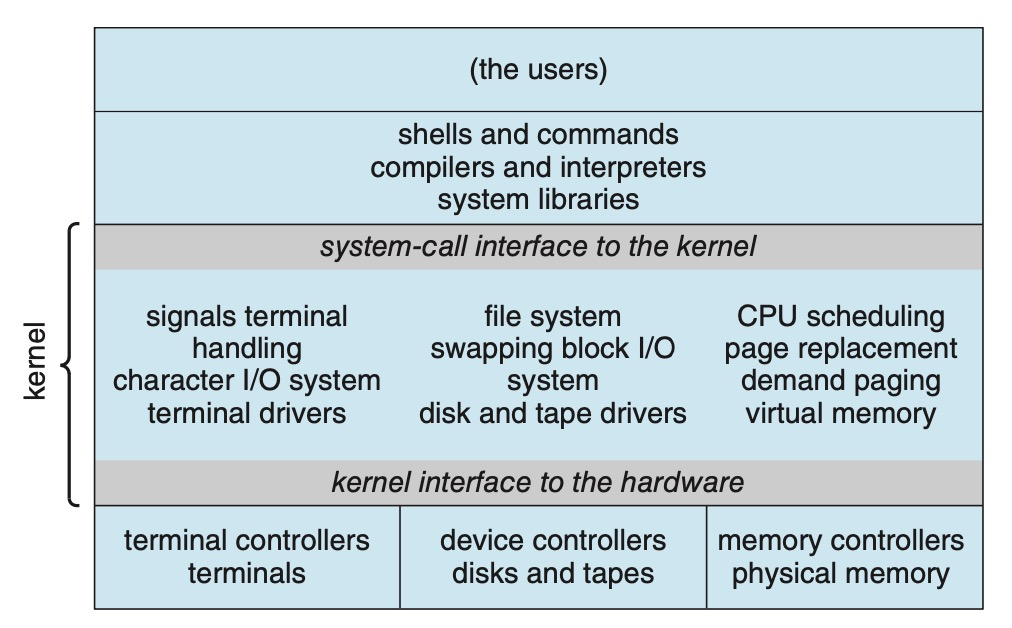
\includegraphics[width=0.55\linewidth]{assets/os-structure.jpg}
\end{figure}

\subsection{Design di un Sistema Operativo}
Abbiamo già visto come vengono definiti gli obiettivi del sistema operativo, vedendo cosa gli utenti e l'hardware si aspettano da esso.

\spacer

Nella progettazione di un software complesso come il sistema operativo è importante mantenere separati i due concetti di politiche e meccanismi.

Le \textbf{politiche} definiscono i compiti e servizi che il sistema operativo deve fornire, mentre i \textbf{meccanismi} definiscono come queste politiche andranno implementate all'atto pratico.

\begin{note}
    In macos e Windows politiche e meccanismi sono fissati a priori e scritti nel sistema, in Linux la separazione tra le due è più evidente.
\end{note}

\subsection{Monolitici}
La struttura più semplice è l'\textbf{assenza di una struttura}. Tutta la funzionalità del kernel viene implementata in un unico eseguibile, con tutte le funzioni strettamente collegate.

\spacer
Questo significa che un singolo bug in uno dei sistemi può comportare il blocco dell'intero sistema, inoltre lo sviluppo e l'estensione risultano essere particolarmente complicati per un kernel monolitico.

Tuttavia quando costruito in modo sicuro la stretta integrazione rende il sistema \textbf{estremamente efficiente}.

\begin{note}
    MS-DOS non implementava una struttura modulare, le applicazioni fanno chiamate a system call direttamente, aprendo così la strada a diverse vulnerabilità.

    \spacer
    Anche UNIX implementava un kernel parzialmente monolitico, con l'obiettivo di migliorare le performance.
    Esso presentava solo due livelli, il kernel e le applicazioni utente. Lo strato del kernel si ritrova con una gran quantità di responsabilità.

    \begin{figure}[H]
        \centering
        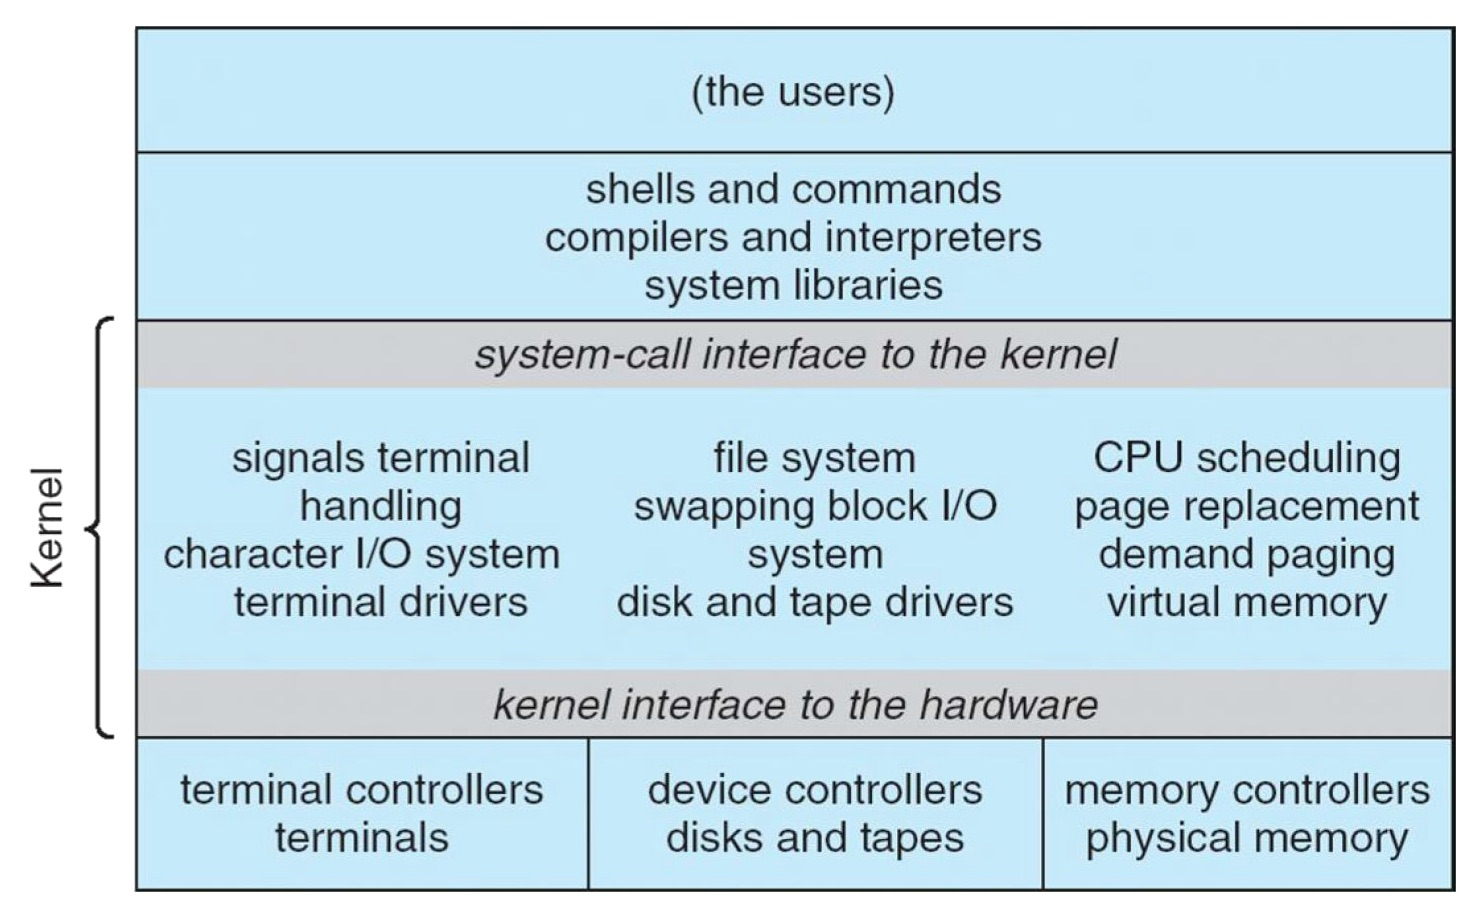
\includegraphics[width=0.5\linewidth]{assets/unix-monolithic.jpeg}
    \end{figure}
\end{note}

\subsection{Approccio stratificato}
L'alternativa all'approccio monolitico è un approccio dove i vari sistemi sono separati in componenti o moduli relativamente piccoli che assieme compongono il kernel.

\spacer
Uno dei modi per implementare un approccio modulare è quello stratificato, in presenza di hardware appropriato è possibile suddividere le funzioni del sistema operativo su vari \textbf{livelli}. Il livello 0 è l'hardware, il livello N è l'interfaccia utente.

Ciascuno strato impiega esclusivamente funzioni degli strati di livello inferiore.

\spacer
Questa struttura ha il vantaggio di facilitare la realizzazione e messa a punto del sistema operativo.

Gli svantaggi invece sono legati ai tempi di attraversamento dei vari strati (si pensi ad una system call che deve essere intercettata e riportata da molteplici livelli) e alla difficoltà di definire gli strati, in quanto essi possono usare solo le funzioni degli strati inferiori (si pensi al driver della memoria virtuale, che dovrebbe essere sopra allo scheduler, perché deve essere possibile interromperne l'esecuzione in caso di page fault. Ma allo stesso tempo lo scheduler deve essere a conoscenza delle informazioni del driver per poter gestire al meglio i processi).

\begin{figure}[H]
    \centering
    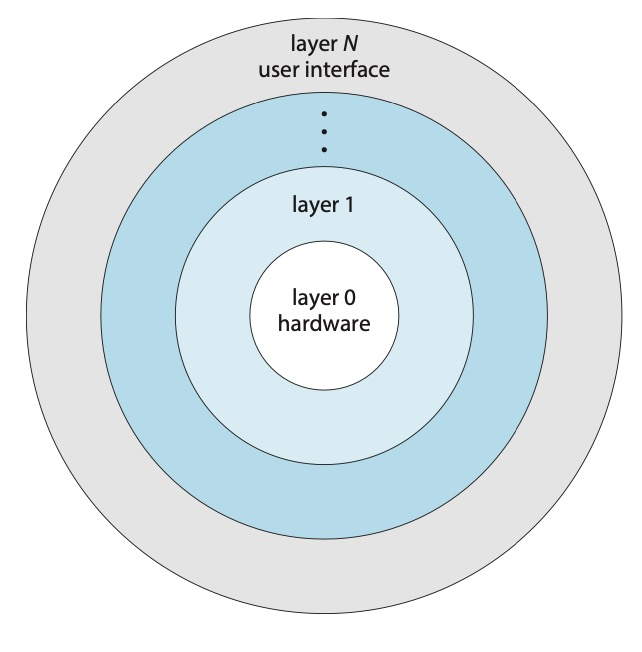
\includegraphics[width=0.4\linewidth]{assets/os-layered.jpg}
\end{figure}

\subsection{Microkernel}
Un microkernel offre la \textbf{minima quantità di servizi} di gestione dei processi, della memoria e di comunicazione.

Tutte le funzionalità non essenziali al kernel sono implementate come programmi utente, c'è quindi necessità di intensa comunicazione tra le varie componenti, cosa che viene mediata dal kernel.

\spacer
Il microkernel è semplice da modificare e rende semplice aggiungere e modificare le funzionalità, in quanto esse sono implementate a livello utente.

Inoltre i sistemi operativi con microkernel sono più sicuri (meno codice viene eseguito a livello kernel) e sono più facili da portare a nuove architetture.

Il più grande svantaggio è l'\textbf{overhead} di prestazioni causato dalle continue comunicazioni tra i moduli.

\begin{figure}[H]
    \centering
    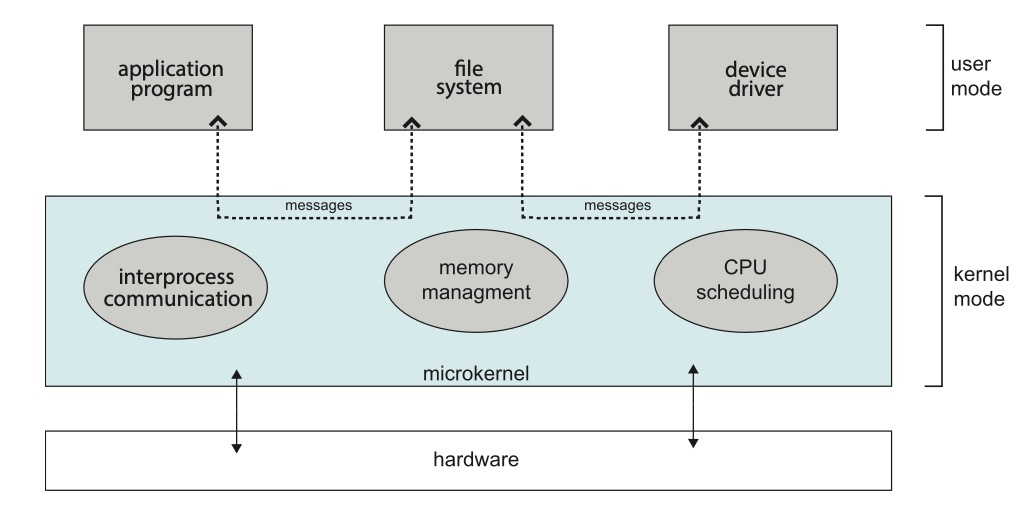
\includegraphics[width=0.5\linewidth]{assets/microkernel.jpg}
\end{figure}

\begin{note}
    Utilizzato da alcuni sistemi operativi più vecchi, come le prime versioni di Windows NT o macOS su kernel darwin.
\end{note}

\subsection{Kernel Modulari}
L'implementazione di tutti i moderni sistemi operativi utilizza i \textit{Loadable Kernel Module (LKMs)}.
Si utilizza un approccio object-oriented dove ciascun modulo implementa un'interfaccia che definisce una funzione del kernel.

Ciascun modulo può comunicare con gli altri moduli mediante l'interfaccia comune, inoltre ogni modulo può essere caricato o meno in memoria in base alle necessità.

\spacer
Questo approccio è simile a quello del microkernel con solo alcuni moduli caricati inizialmente che hanno il compito di caricare gli altri in base alla necessità, ma vengono risolti i problemi di comunicazione.

\subsection{Sistemi ibridi}
Nei sistemi operativi moderni si utilizza spesso un approccio misto rispetto a quelli visti precedentemente.

\subsubsection*{Linux}
Linux ha un kernel principalmente monolitico per poter fornire prestazioni elevate, tuttavia esso può essere anche esteso in modo dinamico.

\subsubsection*{Windows}
Anche Windows è in larga parte monolitico, ma conserva alcune caratteristiche tipiche dei sistemi microkernel tramite il supporto per sottosistemi (\textit{personalities}) che vengono eseguiti a livello utente.

\subsubsection*{macOS e iOS}
Anche se i sistemi possono sembrare molto differenti e vengono eseguiti su architetture e dispositivi diversi, essi condividono una struttura simile.

\spacer
\begin{sitemize}
    \item \textbf{User experience (GUI):} Permette l'interazione col software, diversa per macOS e iOS in base allo stile di input.
    \item \textbf{Ambienti applicativi:} Cocoa fornisce le API per i linguaggi di programmazione Objective-C e Swift.
    \item \textbf{Framework di base:} Ambienti che supportano le API grafiche e di base, come OpenGL.
    \item \textbf{Ambiente kernel:} Darwin include il kernel BSD UNIX, è estendibile grazie ai kext utili allo sviluppo di driver ed estensioni del kernel.
\end{sitemize}
\spacer

Le applicazioni su questi sistemi possono essere progettate per sfruttare le funzionalità di user experience o per aggirarle completamente (disponibile ai developer solo su macOS).

\begin{figure}[H]
    \centering
    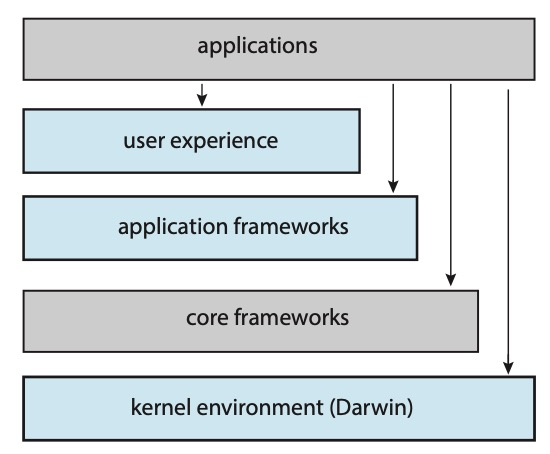
\includegraphics[width=0.4\linewidth]{assets/apple-os-structure.jpg}
    \caption{Struttura dei sistemi macOS e iOS}
\end{figure}

\subsubsection*{Android}
Sviluppato dalla \textit{Open Headset Alliance} di cui Google fa parte, ma non è l'unica grande azienda, Android è un sistema operativo open source che gestisce una gran quantità di dispositivi mobili.

\spacer

Android nasce da una versione modificata del kernel linux, le applicazioni android sono scritte in Java e vengono poi eseguite sull'\textit{Android RunTime (ART)}.
Per migliorare le prestazioni ART non esegue una compilazione a tempo di esecuzione, ma viene eseguita all'installazione dell'applicazione.

Gli sviluppatori possono anche scegliere di utilizzare JNI, l'interfaccia nativa con un accesso più diretto all'hardware.

\begin{figure}[H]
    \centering
    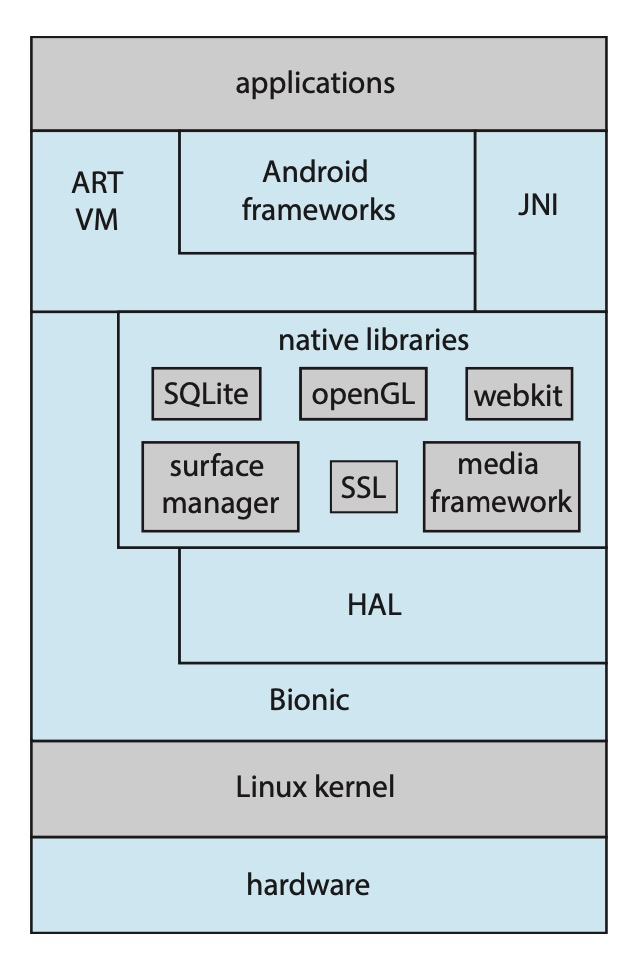
\includegraphics[width=0.27\linewidth]{assets/android.jpg}
    \caption{Struttura sistema android}
\end{figure}

\begin{note}
    Poiché i dispositivi android hanno specifiche hardware pressoché illimitato c'è un livello di astrazione tra l'hardware e le librerie native (\textit{Hardware Abstraction Layer, HAL})
\end{note}
